\section{Linear Algebra}

\subsection{Least-Squares Problem Statement} % (fold)
\label{sub:least_squares_problem_statement}

\begin{definition}[Least Squares]
	Assume matrix A and vectors $\vec{x}$ and $\vec{b}$. The problem defined by
	\[
	\min_{\vec{x}}\|A\v{x}-\v{b}\|^2
	\]
	is a Least Squares Problem (LSP).
\end{definition}

\begin{example}
	Assume we have two dimensional data set $\vec{x}$ and $\vec{y}$ and we want to formalize a LSP to find a linear correlation between x and y. We first formalize the goal linear correlation as
	\[
	y=mx+c
	\]
	where we want to find the optimal values for m and c to minimize the squared loss across all data points. Summarizing the above equation for all data points gives us
	\[
	\begin{bmatrix}
		x_1 & 1\\x_2&1\\\vdots\\x_n&1
	\end{bmatrix}
	\begin{bmatrix}
		m\\c
	\end{bmatrix}=
	\begin{bmatrix}
		y_1\\y_2\\\vdots\\y_n
	\end{bmatrix}
	\]
	Where
	\[
	A = \begin{bmatrix}
		x_1 & 1\\x_2&1\\\vdots\\x_n&1
	\end{bmatrix},\;\;
	\vec{x} = \begin{bmatrix}
		m\\c
	\end{bmatrix}, \;\;
	\Vec{y} = \begin{bmatrix}
		y_1\\y_2\\\vdots\\y_n
	\end{bmatrix}
	\]
	And therefore
	\[
	\min_{\vec{x}}\|A\vec{x}-\vec{b}\|^2 = \min_{m,c}\sum_{i=1}^n(y_i-(mx_i+c))^2
	\]
\end{example}

\begin{theorem}[Ordinary Least Squares]
	Given the column space of the matrix A, for vector $\v{b}$ not in the said column space, $A\v{x}-\v{b} = \v{e}$ must be orthogonal to the columns of A. (Pythagora's theorem)

Therefore, the dot products of every column of A and $\v{e}$ must be zero, i.e.
	\begin{align*}
		A^\top(A\v{x}-\v{b}) &= 0\\
		A^\top A\v{x}-A^\top \v{b} &= 0\\	
		A^\top A\v{x} &= A^\top \v{b}\\
		\v{x} &= (A^\top A)^{-1}A^\top \v{b}
	\end{align*}
We conclude that the solution for Ordinary Least Squares (OLS) is
\[
\v{x}^* = \argmin_{\v{x}}\|A\v{x}-\v{b}\|^2 = (A^\top A)^{-1}A^\top \v{b}
\]
\end{theorem}

% subsection least_squares_problem_statement (end)

\subsection{Norm} % (fold)
\label{sub:norm}

\begin{definition}[Norm]
	A Norm is defined as
	\[
	f:= \mathbf{X}\rightarrow\mathbb{R}
	\]
	For vector space $\mathbf{X}$.

	The norm of x is denoted as $\|x\|$.

	For any vector x and y, we have
	\begin{itemize}
		\item $\|x\|\ge0$ and $\|x\|=0$ iff $x=\v{0}$
		\item $\|x+y\|\le\|x\|+\|y\|$
		\item $\|\alpha x\|=|\alpha|*\|x\|$
	\end{itemize}
\end{definition}

\begin{definition}[l-p Norm]
Generally, l-p norm is defined as
\[
\|\v{x}\|_p := \left(\sum|x_i|^p\right)^{\frac{1}{p}};\;\;1\le p<\infty
\]
Commonly used norms:
\begin{itemize}
	\item $\|\v{x}\|_1 := \sum|x_i|$
	\item $\|\v{x}\|_2 := \sqrt{\sum|x_i|^2}$
	\item $\|\v{x}\|_\infty := \max|x_i|$
\end{itemize}

\end{definition}

\begin{theorem}[Cauchy-Schwartz Inequality]
	\[
<\v{x}, \v{y}> = \v{x}^\top\v{y} = \|\v{x}\|_2\|\v{y}\|_2\cos \theta
	\]
	Since $-1 \le \cos \theta \le 1$,
	\[
<\v{x}, \v{y}> = \v{x}^\top\v{y} \le \|\v{x}\|_2\|\v{y}\|_2
	\]
\end{theorem}

\begin{theorem}[Holder's Inequality]
For $p,q\ge1 \;\;\t{s.t.}\;\; \frac{1}{p}+\frac{1}{q}=1$,
\[
|\v{x}^\top\v{y}|\le \sum_{i=1}^n|x_iy_i|\le \|\v{x}\|_p\|\v{y}\|_p
\]
i.e., Cauchy-Schwartz is a narrowed case of Holder's Inequality.
\end{theorem}

% subsection norm (end)

\subsection{Gram-Schimdt} % (fold)
\label{sub:gram_schimdt}

\begin{theorem}[Gram-Schimdt/QR-decomposition]
	Let X be a vector space with basis \{$\li{\v{a}}{n}$\}, which is orthonormal.
	For any matrix A,
	\begin{align*}
		A &= QR\\
		\begin{bmatrix}
			\li{\v{a}}{n}
		\end{bmatrix} &=
		\begin{bmatrix}
			\li{\v{q}}{n}
		\end{bmatrix}
		\begin{bmatrix}
			\v{r}_{11} & \v{r}_{12} & \cdots & \v{r}_{1n}\\
			0 & \v{r}_{22} & \cdots & \v{r}_{2n} \\
			0 & 0 & \ddots & \v{r}_{3n} \\
			0 & 0 & 0 & \v{r}_{nn}
		\end{bmatrix}
	\end{align*}
	Where Q is orthonormal andR is upper-triangular.
\end{theorem}

\begin{theorem}[Fundamental Theorem of Linear Algebra]
For matrix $A\in \mathbb{R}^{m*n}$,
	\[
Null(A)\bigoplus Range(A^\top) = \mathbb{R}^n
	\]
Where $\bigoplus$ denotes "direct sum" and $Range(A^\top)$ is the column space of $A^\top$. With the said equation we can also conclude that
\[
Range(A)\bigoplus Null(A^\top) = \mathbb{R}^m
\]
\end{theorem}

\begin{theorem}[orthogonal decomposition theorem]
X a vector space and S a subspace of X. Then for any $\v{x}$ in X,
\[
\v{x} = \v{s} + \v{r}, \;\; \v{s} \in S,\;\; \v{r} \in S^\perp
\]
Such that
\[
S^\perp = \{\v{r}\;|<\v{r}, \v{s}>\;=0,\;\; \forall \v{s}\in S\}
\]
Therefore, 
\[
\mathbf{X} = S\bigoplus S^\perp
\]
\end{theorem}

\begin{example}[Minimum Norm Problem]
	We want to find
	\[
\min \|\v{x}\|_2^2
	\]
	subject to $A\v{x}=\v{b}$.
	From FTLA we know that
	\[
\v{x} = \v{y}+\v{z}\;\;s.t.\;\;\v{y}\in N(A;\;\;\v{z}\in R(A^\top).
	\]
	And
	\[
A(\v{y}+\v{z}) = 0 + A\v{z} = \v{b}
	\]
	Since $\v{y} \perp \v{z}$,
	\[
\|\v{x}\|_2^2 = \|y\|_2^2+\|z\|_2^2
	\]
	Consider $\v{z} = A^\top\v{w}$, 
	\begin{align*}
		A\v{z} &= \v{b}\\
		AA^\top\v{w} &= \v{b}\\
		\v{w} &= (AA^\top)^{-1}\v{b}
	\end{align*}
	Therefore
	\[
\v{z} = \min{\|\v{x}\|_2^2} =  A^\top(AA^\top)^{-1}\v{b}
	\]
\end{example}

% subsection gram_schimdt (end)

\subsection{Symmetric Matrices} % (fold)
\label{sub:symmetric_matrices}

\begin{definition}
	Matrix A is symmetric if $A=A^\top$, i.e. $A_{ij} = A_{ji}$. 

	Set $\mathbb{S}^n$ means the set of symmetric matrices of dimension n.
\end{definition}

\begin{theorem}[Spectral Theorem]
	If matrix A $\in \mathbb{S^n}$, then
	\begin{itemize}
		\item All eigenvalues of A are real numbers
		\item Eigenspaces are orthogonal
		\item $dim(N(\lambda_iI-A))=\mu_i$ where $\mu_i$ is the algebraic multiplicity of $\lambda_i$
	\end{itemize}
	This means that A is always diagonalizable. i.e.:
	\[
	A = U\Lambda U^\top
	\]
	where U orthonormal and $\Lambda$ diagonal. Orthonormal (or, unitary) means that the columns of U are orthogonal and all columns are normalized, i.e.
	\[
	U^{-1} = U^\top
	\]
\end{theorem}

\begin{theorem}
	For a diagonalizable n*n matrix A that has n linearly independent eigenvectors, A can be factorized as
	\[
A = U\Lambda U^\top
	\]
	Where U orthonormal and $\Lambda$ is a diagonal matrix consists of the eigenvalues of A such that
	\[
\Lambda = \begin{bmatrix}
	\lambda_1 & & \\
	& \ddots & \\
	& & \lambda_i
\end{bmatrix}
	\]
	Therefore it is also called an eigenvalue decomposition.
\end{theorem}

% subsection symmetric_matrices (end)

\subsection{Principal Component Analysis} % (fold)
\label{sub:principal_component_analysis}

\begin{definition}
	For $A\in\mathbb{S}$, its Rayleigh coefficient is defined as
	\[
R = \frac{\v{x}^\top A\v{x}}{\v{x}^\top\v{x}}
	\]
	The Rayleigh coefficient can bound the eigenvalues of A such that,
	\[
\lambda_{min}(A) \le \frac{\v{x}^\top A\v{x}}{\v{x}^\top\v{x}} \le \lambda_{max}(A)
	\]
	PCA is very similar to Singular Value Decomposition (SVD). SVD has more nice properties than PCA.
\end{definition}

% subsection principal_component_analysis (end)


\subsection{Singular Value Decomposition} % (fold)
\label{sub:singular_value_decomposition}

\begin{theorem}[SVD]
	Let $A \in \mathbb{R}^{m*n}$, the SVD of A is given as
	\[
A = U \Sigma V^\top
	\]
	Where
	\[
	U\in\mathbb{R}^{m*m},\;\; \Sigma\in\mathbb{R}^{m*n},\;\;V\in\mathbb{R}^{n*n}
	\]
	and $\Sigma$ has real entries in its diagonal (the singular values) and zero's else where.
	If $Rank(A)=r$, we can rewrite A as
	\[
A = \sigma_1\v{u}_1\v{v}^\top_1 + \sigma_1\v{u}_1\v{v}^\top_1 + \cdots + \sigma_r\v{u}_r\v{v}^\top_r
	\]
\end{theorem}

\begin{remark}[geometric interpretation of SVD]
	Consider linear transformation on vector $\v{x}$ given by matrix A, s.t.
	\[
	A\v{x} = U \Sigma V^\top \v{x}
	\]
	SVD helps breaking the transformation into three smaller steps, i.e.
	\begin{itemize}
		\item orthonormal transformation (rotate/reflect) by V,
		\item scaling by $\Sigma$,
		\item orthonormal transformation by U.
	\end{itemize}
	The following illustration is an example of a 2D transformation $A\v{x}$. It shows the decomposed linear transformation through the unit circles relative to the original unit circle at different stages of the transformation.\\
	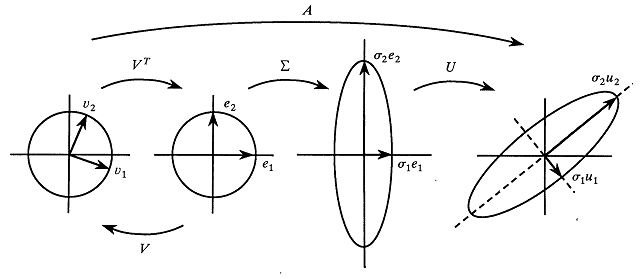
\includegraphics[scale=0.7]{img/svd1.png}
\end{remark}

\begin{theorem}[Proof of SVD]
	For $A\in\mathbb{R}^{m*n}$, consider symmetric matrix $A^\top A$ that has eigenvalues $\lambda_1 \cdots \lambda_r > 0$ with corresponding eigenvectors $v_1 \cdots v_r$ and $\lambda_{r+1} \cdots \lambda_n = 0$. Then we know that
	\[
	A^\top A\v{v}_i = \lambda_i\v{v}_i
	\]
	Let
	\[
	V = \begin{bmatrix}
	| & & | \\
	\v{v}_1 & \cdots & \v{v}_n\\
	| & & |
	\end{bmatrix}
	\] 
	Define $\sigma_i = \sqrt{\lambda_i}$, let 
	\[
A\v{v}_i = \sigma_i\v{u}_i \;\; i\le r
	\]
	for some vector $\v{u}_i$. \\ 

	\textbf{Claim.} $\v{u}_i$ are orthonormal.
	\begin{proof}
	\begin{align*}
		\v{u}_i^\top\v{u}_j &= \frac{(A\v{v}_i)^\top}{\sigma_i}\frac{(A\v{v}_j)}{\sigma_j} \\
		&= \frac{1}{\sigma_i \sigma_j}\v{v}_i^\top A^\top A \v{v}_j && A^\top A\v{v}_j = \lambda_j\v{v}_j\\
		&= \frac{1}{\sigma_i \sigma_j}\v{v}_i^\top \lambda_j\v{v}_j \\
		&= \frac{\lambda_j}{\sigma_i \sigma_j}\v{v}_i^\top \v{v}_j && \v{v}_i \v{v}_j \text{ orthonormal}\\
		&= \left\{\begin{array}{lr}
			0 & i\neq j \\
			1 & i =j
		\end{array}
	\end{align*}
	Therefore $\v{u}_i$ are orthonormal.
	\end{proof}
	Recall that A has rank r, we let
	\[
V_r = V = \begin{bmatrix}
	| & & | \\
	\v{v}_1 & \cdots & \v{v}_r\\
	| & & |
	\end{bmatrix}
	\]
	Hence
	\begin{align*}
		AV_r &= 
	\begin{bmatrix}
	| & & | \\
	\v{u}_1 & \cdots & \v{u}_r\\
	| & & |
	\end{bmatrix}\begin{bmatrix}
	\sigma_1 & & \\
	 & \ddots & \\
	 & & \sigma_r
	\end{bmatrix} = U_r\Sigma_r\\
	A&= U \Sigma V^\top
	\end{align*}
	Since V orthonormal and $V^{-1}=V^\top$
\end{theorem}

% subsection singular_value_decomposition (end)

\subsection{Low-Rank Approximation} % (fold)
\label{sub:low_rank_approximation}

\begin{definition}[matrix norms]
There are two ways to interpret a matrix, either as an operator or as a block of data. Frobenius norm consider the matrix as a block of data.
	
	\noindent\textbf{Frobenius norm} of matrix A is defined as
	\[
\|A\|_F = \sqrt{\sum_{i=1}^m\sum_{j=1}^na_{ij}^2} = \sqrt{tr(A^\top A)}
	\]
	Frobenius norm is invariant to orthonormal transformations, i.e. given U an orthonormal matrix,
	\[
\|UA\|_F = \|AU\|_F = \|A\|_F
	\]

	\noindent\textbf{Spectral norm}, or $l_2$ norm, interpret the matrix as an operator and is defined as
	\[
\|A\|_2 = \max_{\|\v{x}\|_2=1}\|A\v{x}\|_2 = \max_{\|\v{x}\|=1}\sqrt{\v{x}^\top A^\top A\v{x}} = \sqrt{\lambda_{max}(A^\top A)} = \sigma_{max}(A^\top A)
	\]
	Intuitively, the spectral norm of a matrix A is the largest scaling that A can do (recall the $\Sigma$ matrix that is used to scale the unit circle in the three steps of transformation after SVD).
\end{definition}

\begin{theorem}[Eckart-Young-Mirsky Theorem]
	$A \in \mathbb{R}^{m*n}$. Do SVD gives us
	\[
A = U \Sigma V^\top = \sum_{i=1}^n \sigma_i\v{u}_i\v{v}_i^\top
	\]
	Define
	\[
A_k = \sum_{i=1}^k \sigma_i\v{u}_i\v{v}_i^\top
	\]
	We want to find the best k-rank (lower than r) approximation of A, i.e.
	\[
\argmin_{B\in \mathbb{R}^{m*n},\;Rank(B)=k}\|A-B\|_F
	\]
	Suprisingly, Eckart-Young-Mirsky Theorem tells us that
	\[
\argmin_{B\in \mathbb{R}^{m*n},\;Rank(B)=k}\|A-B\|_F = A_k
	\]
	Moreover,
	\[
\argmin_{B\in \mathbb{R}^{m*n},\;Rank(B)=k}\|A-B\|_2 = A_k
	\]
	This theorem relates two completely different norms and is not obvious at all. It shows how fundamental SVD is, such that in any way of looking at a matrix, the decomposition shows up.
\end{theorem}

\begin{remark}
	Eckart-Young-Mirsky Theorem can be used to \textbf{compress images}. For an image, the matrix that represents the pixels of the image can be reduced to a lower rank matrix, and hence a smaller set of data, while remains relatively high resolution. The $A_k$ matrix \textbf{captures the key features of the image because it keeps $k$ largest singular values and their corresponding vectors that contribute most to the dataset/transformation.}
\end{remark}

\begin{definition}[trace]
	The trace of a matrix is defined as
	\[
	trace := \mathbb{R}^{n*n} \rightarrow \mathbb{R}
	\]
	\[
trace(A) = \sum_{i=1}^na_{ii}
	\]
\end{definition}

\begin{remark}[Orthonormal transformation invariance of Frobenius norm]
	Proof that $\|UA\|_F = \|AU\|_F = \|A\|_F$
	\begin{proof}
		Recall that $\|A\|_F = \sqrt{tr(A^\top A)}$. By definition, for any matrices A and B, we have $tr(AB)=tr(BA)$ Then,
		\begin{align*}
			\|AU\|_F &= \sqrt{tr((AU)^\top(AU))}\\
			&= \sqrt{tr(U^\top A^\top AU)}\\
			&= \sqrt{tr(UU^\top A^\top A)}\\
			&= \sqrt{tr(A^\top A)}\\
			&= \|A\|_F
		\end{align*}
	\end{proof}
\end{remark}

\begin{remark}[Frobenius norm is the sum of singular values]
\begin{align*}
	\|A\|_F &= \|U \Sigma V^\top\|_F = \|\Sigma\|_F\\
	&=\sqrt{\sum_{i=1}^n \sigma_i^2}
\end{align*}
\end{remark}

% subsection low_rank_approximation (end)

